\chapter{Постановка задачи и обзор существующих методов}
\subsection{Белок-белковое взаимодействие}
Рассмотрим белок, имеющий четвертичную структуру.

\textbf{Вопрос}: можно ли изменить что-то в его структуре, чтобы образующие его цепочки были лучше сцеплены между собой?

Пусть есть комплекс из двух белков (например, имунноглобулин и эпитоп).

\textbf{Вопрос 1}: можно ли изменить что-то в его структуре, чтобы усилить связь между компонентами комплекса?

\textbf{Вопрос 2}: насколько специфична одна из компонент комплекса?  Можно ли подобрать один из белков так, чтобы комплекс был более устойчивым? Насколько заменяема каждая из компонент?

Ответить нам поможет \textbf{аланиновое сканирование} (аланиновый мутагенез).
\section{Аланиновое сканирование}
Аланиновое сканирование (ала-скан)~\cite{alascan2001} - метод для определения аминокислот в составе белка, играющих важную роль в сохранении его функций, стабильности или формы.
\begin{wrapfigure}{RT}{0.3\textwidth}
\resizebox{0.3\textwidth}{!}{
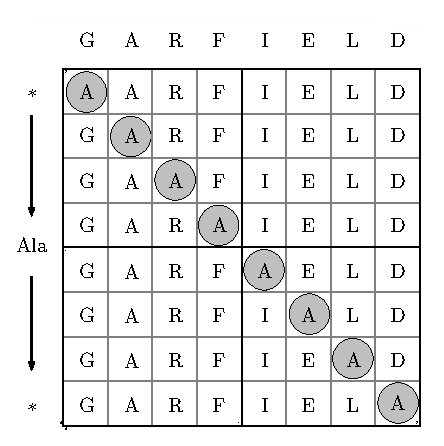
\includegraphics{ala_scan.eps}
}
\end{wrapfigure}
\subsection{Аланиновое сканирование in vitro/in vivo}
Проблемы ala-scan in vitro/in vivo:
\begin{itemize}
\item Большое пространство поиска.
\item Сложность синтеза библиотек: необходим индивидуальный подход!
\item Высокая стоимость.
\end{itemize}
\subsection{Аланиновое сканирование in silico: решаемые задачи и границы применимости}
написать про метод, протоколы, используемые функции, что такое дельта-дельта G

сказать, что в данной работе используется протокол из rosetta (мб привести картинку про реальную ddG и in silico функцию изменения энергии), сцепленность цепочек оценивается в смысле изменения энергии, применяемый в протоколе метод монте-карло лежит за пределами работы (кроме того, является относительно хорошо изученным, в ходе работы никакие модификации в сам метод или функцию оценки ddG не вносились), поэтому не приводится. 
\section{Стандартные методы выбора аминокислот для аланинового сканирования in silico}

Как правило, при компьютерном моделировании аланинового сканирования применяют предварительную фильтрацию аминокислот, после которой проводится сканирование. Для фильтрации используются два основных метода~\cite{hotspots2012rev}:
\begin{itemize}
\item отсечка по расстоянию ~\cite{kortemme2004}: мутации подвергаются только те аминокислоты, которые расположены вблизи области взаимодействия пары белков;

\item выбор по гомологии: аминокислоты выбираются исходя из имеющихся экспериментальных результатов аланинового сканирования, проводившихся на близких (в эволюционном смысле) последовательностях.
\end{itemize}

Посмотрим, насколько эффективны эти подходы.

\subsection{Использование отсечки по расстоянию}

\begin{itemize}
\item Аланиновому сканированию подвергаются аминокислоты цепочки, образующей комплекс совместно с другой цепочкой, содержащие атомы, удаленные от каких-либо атомов цепочки, также участвующей в образовании комплекса, на расстояние, не превышающей некоторой фиксированной величины

\item В качестве порогового значения расстояния используются, например, величины 4, 5, 8 \AA{}

\item в Rosetta Alascan Protocol используется усложнение: дополнительно рассматриваются аминокислоты, $\beta$-углерод которых после формирования комплекса в шаре определенного фиксированного радиуса содержит существенно больше атомов $\beta$-углерода, чем содержал до этого.
\end{itemize}
Эксперимент
\begin{itemize}
\item Рассмотрим базу данных с информацией о результатах эспериментов по аланиновому сканированию белков ASEdb~\cite{asedb2001}.
\item Найдем объекты с корректными ссылками на записи в Protein Data Bank ~\cite{rcsb}.
\item Среди всех таких объектов, найдем те, в которых есть аминокислоты, мутация которых приводит к существенному изменению свободной энергии комплекса ($\geq 1$ ккал/моль)
\item Посмотрим, всегда ли они удалены от интерфейса в пределах стандартно используемой отсечки (в качестве примера возьмем расстояние, не превышающее 8 \AA{}).
\end{itemize}

\resizebox{0.8\textwidth}{!}{
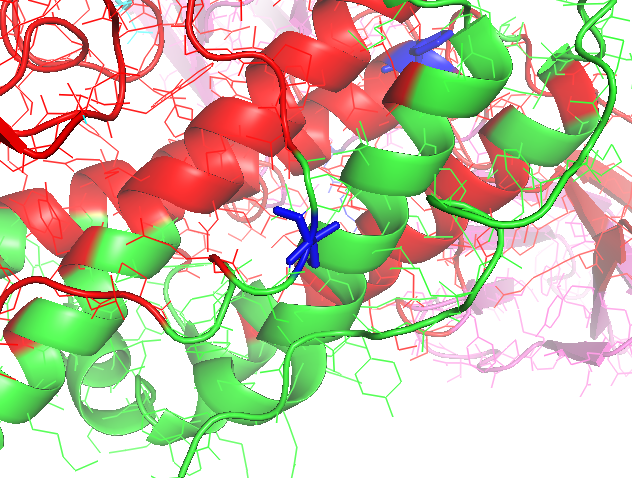
\includegraphics{image7.png}
}

\subsection{Поиск по гомологии}

